\chapter{Analysis of Flow Cytometry Data}
\label{chap:two}
The following chapter introduces the reader to basic information about flow cytometry, its origin, underlying mechanisms, and its use in academic and medical settings. The reader is acquainted with flow cytometry data analysis techniques. 

\section{Introduction to Flow Cytometry}
\label{sec:introtoflow}
Flow cytometry is a high-throughput laboratory technique that allows for studying cellular populations, and is used for hypothesis testing as well as in the medical areas in both biomedical research and diagnostics, most importantly in clinical immunology. As described in \cite{black2011cell}, cell-based screening also facilitates the development of safer and more effective drugs. 

Flow cytometry is non-destructive.

\paragraph{Goals}
\label{sec:flowgoals}
Flow cytometry aims to analyze the physical and chemical features of small particles. In a biological context, the particles are usually various cells, although they can also be bacteria \citep{steen2000flow, nebe2000analysis}. 
By using the flow cytometry technique, one can expect to see the division of input cell population according to various parameters, such as extracellular vesicles \citep{nolan2015flow}, membrane proteins \citep{schmitz2021bimolecular}, antibodies \citep{kalina2020relevance, hall1996use}, and intracellular particles \citep{pirone2021three, wronska2022intracellular}. Using flow cytometry for measurements of molecular interactions such as ligand binding \citep{nolan1998emergence} or protein phosphorylation state \citep{perez2002simultaneous} is possible.

Flow cytometry has facilitated access to new intracellular pathways, which were not revealed by other biochemical approaches \citep{sachs2005causal}.

\paragraph{History}
\label{sec:flowhistory}
Flow cytometry was developed to suit the need to analyze cells and other particles. The prototypal development started in the 1940s with the invention of a device known as Coulter counter. The Coulter counter was a small device that relied on particles flowing in a conducting fluid. The movement was directed by an electrical field, which produced a measurable electrical impedance, through which it was possible to measure the size and number of cells \citealp{graham2013coulter}. The idea has been improved ever since then, focusing mainly on the three underlying physical systems: fluidics, optics, and electronics. Each of the improvements led to more precise measurements \citep{picot2012flow}. There were many growth opportunities for the Coulter counter, such as the development of a multichannel solution or the replacement of the analog electrical circuit with a digital one. Flow cytometry was built upon the foundation of the Coulter counter. 

The principle can be best described by figure \ref{fig:twofeat} and the legend as the author specifies: "When stopcock F is opened,
the mercury in the manometer reservoir R is drawn upward by
a small vacuum pump connected to P, and the resulting pressure
head causes movement of mercury column J after the stopcock is
closed, drawing sample suspension E from the sample vessel
through the hole in aperture wafer A into sample tube B. The
aperture wafer and sample tube are made of dielectric materials
having an electrical resistivity much greater than that of the
suspending medium. Via connections H and I, electrodes C and D
couple an electrical current through the aperture, and the resultant
signal pulses to an amplifier and pulse counter (not shown). The
volume of sample to be analyzed is determined by three control
electrodes (K, L, M) penetrating the wall of the manometer
tubing; when the flowing mercury causes electrical contact between K and L, the pulse counter starts, while mercury contact
with M at a calibrated distance from L terminates it. Thus, cells
are only counted in suspension flowing through the aperture
at constant velocity, so permitting cell concentration to be determined as the count in the suspension volume equal to the
volume of mercury between the electrodes L and M. The second
stopcock G is only opened to fill or flush the sample tube with
clean suspending media via O. The microscope for viewing the
aperture is not shown." (Taken from \cite{don2003coulter}.)

    \begin{figure}[h!]
        \centering
        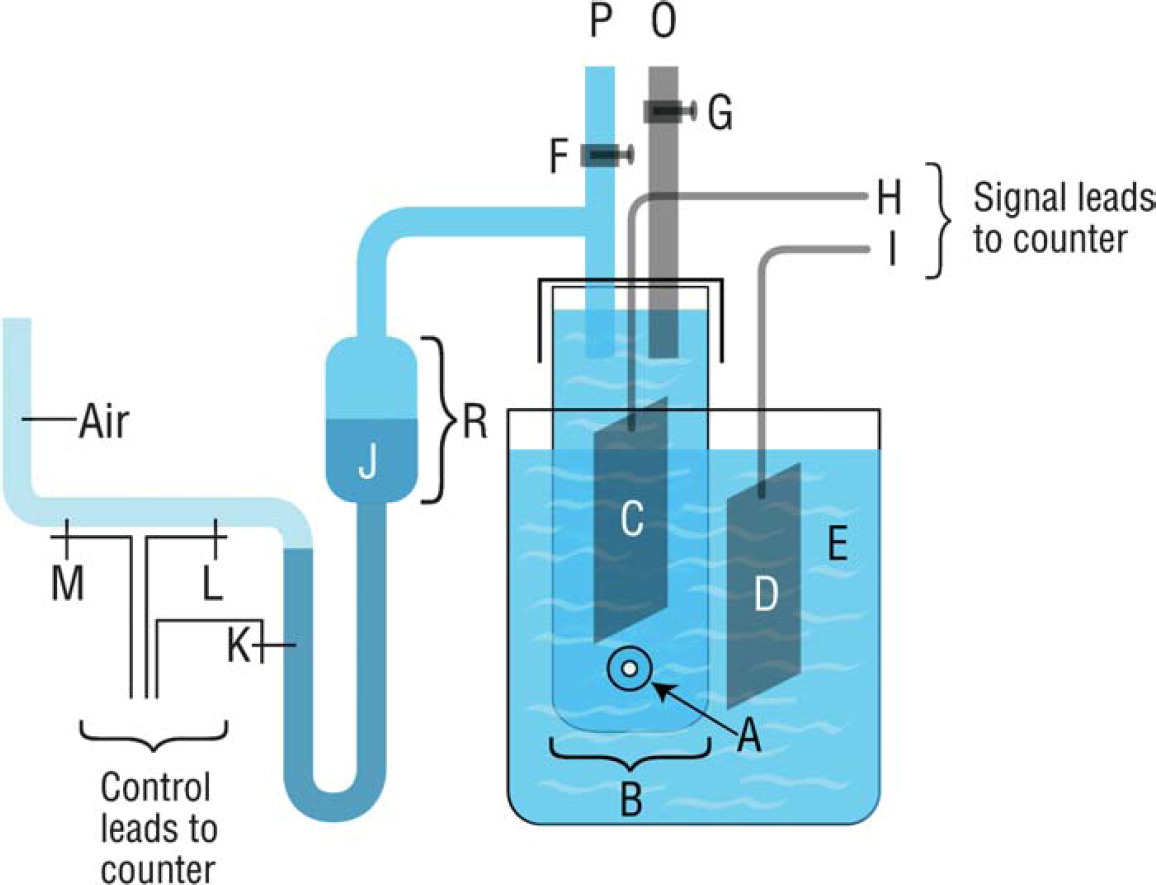
\includegraphics[width=0.9\textwidth]{Figures/coulter.jpeg}
        \caption{Schematic of the Coulter sample stand taken from \cite{don2003coulter}.} 
        \label{fig:twofeat}
    \end{figure}


\paragraph{Principle}
\label{sec:flowprinc}
Three main physical systems come into play: fluidics, optics, and electronics. 

Fluidics is responsible for directing the suspended particles through a flow cell, in which the optical part of the cytometer operates. The flow of the particles needs to be controlled, steady and predictable. The cells need to be sorted and directed. A well-designed system can leverage fluidics to prevent clogging and blockages. Today, one can talk about microfluidics rather than fluidics. Microfluidics operates at much smaller scales, bringing the necessary dimensions down to micrometers, promising a new, more portable and precise generation of devices \citep{gong2019new}.

Optics is responsible for creating scattered light or emitted fluorescence, which carry information about the cells count, granularity, or chemical composition. Parts of the optical system are lenses that shape and focus lasers beams and lasers to provide a source of light \citep{adan2017flow}.

In the past, the lasers were noble gas lasers, and that meant mostly argon-ion lasers \citep{kamentsky1991microscope}. Later, cytometers were updated so they can take advantage of solid-state lasers. The advantage of lasers over different light sources is that the illumination point can easily be focused. The light scatters of individual cells flowing in a stream, targeting small sample volumes at a time, leading into sorting cells by size and complexity, cell cycle, or cell viability. Cells can be tagged with dyes or antibodies \citep{wilkerson2012principles}. The usage of multiple lasers is possible \citep{bigos1999nine, de2016quantification, ashcroft2000commercial}. A comprehensive overview of lasers in flow cytometry can be found in \cite{shapiro2018lasers}.

Electronics is responsible for detecting signals from flow cytometry. A useful tool is called discriminator, which is a circuit that can be aimed at specific voltages thus preventing circuit overload. Amplifiers are used to produce signals, translating the input into information. The electronic systems can take advantage of more complicated parts as explained in \cite{robinson2004flow}.

\paragraph{Tools}
\label{sec:flowtools}
A device used for the flow cytometry technique is called a flow cytometer. Flow cytometers can go through thousands of samples a day.

Commercially sold flow cytometers can be sorted into two categories: analysers or sorters. As the name suggests, sorters both collect data and sort cells by their properties. Flow cytometers can also be adjusted to specific use cases, such as the Ploidy Analyser manufactured by Partec, which is mainly targeted at analyzing plant material as plants are regularly polyploid - meaning they have at least three complete sets of chromosomes \citep{zhang2003genetic, jacob1998pollen, geng2011genetic}. 

However, improvements such as the development of new fluorescent dyes led to a massive increase in dataset size. Having more colors at one's disposal allows for tracking more parameters at a time, creating a subtechnique of flow cytometry known as polychromatic flow cytometry. ???? intracellular parameters, producing rich information about individual cells \citep{wood20069}, that is impossible to process in traditional manual ways such as sequential manual gating, which is also observer-dependent and requires high specialization, often impacting results. It is also incredibly time-consuming. The lack of a fully functional automated tool hinders the full potential of flow cytometry. 

To deal with the high-dimensional data and the issue of evergrowing time and space requirements, computer-driven analytical techniques have been introduced, especially but not only from the area of hierarchical clustering as described in section \ref{sec:hierarchicalclustering}.

Methods that are reliant on prior knowledge of expected cell populations (clusters) \citep{lo2008automated, rogers2008cytometric, wilkins2001comparison, zeng2007feature} to deal with automatization and move the thing to the less observer-dependent manner are often. 

\section{Analysis}
\label{sec:analviagating}
Several methods of flow cytometry dataset analysis will be described in this section.
The analysis of data obtained from a flow cytometer can be done manually with all of its possible downfalls, or with the help of either commercially or freely available software. 

As with other types of workflows, quality assessment and control is essential. Through quality assessment, one can make sure that the differences among samples are biological, not technical. One of the approaches which can solve the issue is the development of graphical tools which can reveal non-biological differences among samples \citep{le2007data}. Other methods suggested calibrating computation for each of the fluorescent parameters \citep{gratama1998flow}.

\paragraph{Gating}
\label{sec:gating}
Gating is a method that creates subsets of particles based on the flow cytometer output. Gating works by using defined regions called "gates". Gates can be of various dimensions and shapes.

Sequential gating is a subtechnique of gating and is useful for the identification of specific populations. Sequential gating differs from regular gating in terms of the number of used gates and the order in which the gates were used. In sequential gating, each gate refines the population selection, starting with removing background noise. Gates can be added or tweaked in order to include or exclude data based on various parameters such as size or fluorescence intensity. Alas, it is limited in its visualization capabilities, as it can only take one as far as two parameters simultaneously. It is also prone to observer-dependent errors \citep{herzenberg2006interpreting}.

Due to the algorithmic nature of gating, it's a process that can be automated. Automation has a couple of advantages including human error prevention. However, automated gating difficulty increases with nonconvex cell populations, meaning populations that are neither concave nor convex but rather they curve up and down, or other multidimensional shapes, and can struggle with elliptical shapes that are often produced from flow cytometry \cite{finak2009merging}.

\paragraph{Probability Binning}
\label{sec:probabilitybinning}
Probability binning can help identify differences that are not visible through sequential manual gating by distributing the data into bins of the same size and comparing the count of events between the experimental sample and the control sample. While historical methods that include Overton subtraction \citep{overton1988modified} or Komogorovs-Smirnoff statistic \citep{young1977proof} were useful, they suffered from enormous counts of bins. Probability binning works by minimizing the maximum expected variance by creating bins of various sizes. The smaller the bins, the more events, however, at the end, each bin no matter its size houses the same amount of events. It then compares the distributions and does not require setting the expected number of cell populations from the beginning. One of its main advantages is that its computation time does not increase with scaling to more parameters. With quality assessment, it can escape one of its major downfalls, which is the sensitivity to variation in experimental conditions.

Frequency difference gating (also known as frequency subtraction gating) takes advantage of probability binning and aims to find and identify rare populations. An example application of frequency difference gating can be found in \cite{roederer2001frequency}.

\paragraph{Cluster Analysis}
\label{sec:clusteran}
Due to the nature of this thesis, cluster analysis is described in depth in \ref{sec:hierarchicalclustering}. 
One does not have to work with high-dimensional data when they can get rid of the dimensions via principal component analysis. Principal component analysis is an unsupervised method of dimension-reduction, which works by creating a new dataset in which the new variables - principal components - are linear combinations of the original values. This allows for detecting patterns \citep{rauber2021cerebrospinal}.

Both principal component analysis and cluster analysis also have the advantage of being able to take fluorescent values individually and therefore account for individual variation.

